\label{execution}
%%%%%%%%%%%%%%%%%%%%%%%%%%%%%%%%%%%%%%%%%%%%%%%%%%%%%%%%%%%%%%%%%%
%%%%%%%%%%%%%%%%%%%%%%%%%%%%%%%%%%%%%%%%%%%%%%%%%%%%%%%%%%%%%%%%%%

\subsection{Introduction}
Quand un ordinateur est allumé, un signal est envoyé à la carte mère qui démarre
l'alimentation. Le processeur démarre alors en mode réel (16 bits). Un signal
est ensuite envoyé pour charger le \acrshort{bios}. Le \acrshort{bios} est le
\textit{firmware} du \acrshort{pc}, il est localisé en mémoire flash de la carte
mère. Il a pour rôle de vérifier que chaque périphérique est alimenté et qu'il
n'y a pas de problème avec la mémoire puis il initialise le \textit{hardware}.
Ensuite, le \acrshort{bios} charge le \acrshort{mbr} depuis le premier disque.
Le \acrshort{mbr} est situé dans les 512 premiers octets du disque et il contient
le \textit{bootloader} du système qui est un morceau de code exécutable. Le
\textit{bootloader} a pour tâche de localiser l'image du \textit{kernel} pour le
charger en mémoire. Il passe ensuite le \acrshort{cpu} en mode protégé (32 bits) 
puis exécute le code du \textit{kernel}. La figure \ref{fig:exec:boot} résume tout
ce processus appelé \textit{boot} en anglais \cite{ref42}.

\begin{figure}[!h]
  \centering
  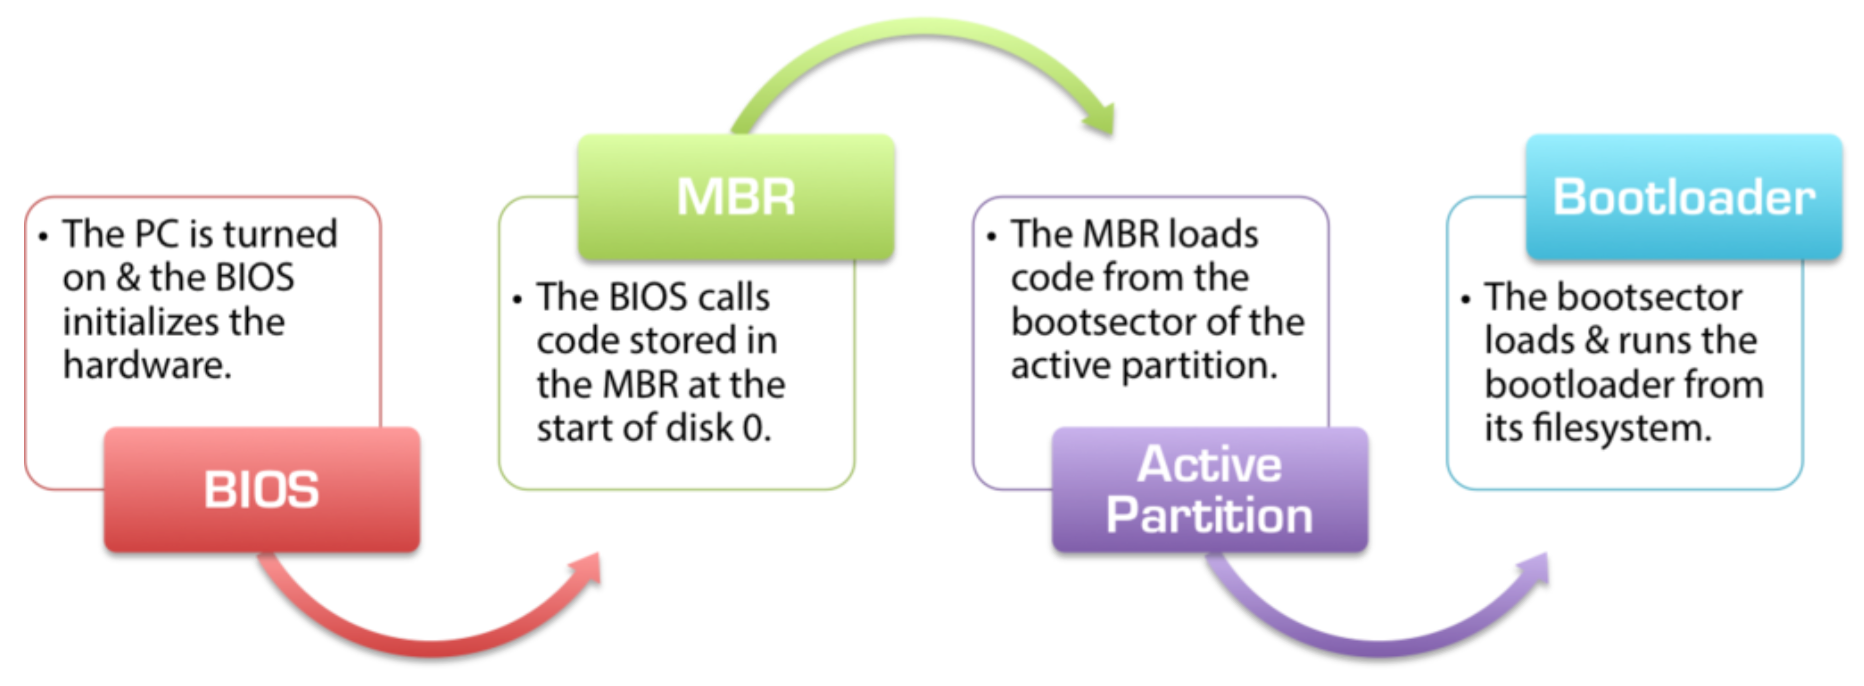
\includegraphics[scale=.45]{images/bios_boot.png}
  \caption{\textit{Boot} d'une machine à base de \acrshort{bios}}
  \label{fig:exec:boot}
\end{figure}

Pour rappel, nous utilisons le logiciel QEMU, qui émule le comportement d'une
machine physique. Pour exécuter notre \textit{kernel} sur QEMU, il faut d'abord
compiler ses sources en un exécutable au format \acrshort{elf}. Une image \acrshort{iso}
doit ensuite être générée à partir de ce fichier. Cette image doit contenir le
\textit{kernel} et le \textit{bootloader} de notre système d'exploitation.
Il est possible d'écrire son propre \textit{bootloader} mais c'est une démarche
assez complexe. Il existe de nombreux \textit{bootloaders open source}. Celui
utilisé dans ce projet est \acrshort{grub}. L'exécution du \textit{kernel} se
déroule donc en deux parties. Il faut dans un premier temps compiler tout le code
du \textit{kernel} puis créer un fichier image à partir du \textit{kernel}
compilé et de \acrshort{grub}.

%%%%%%%%%%%%%%%%%%%%%%%%%%%%%%%%%%%%%%%%%%%%%%%%%%%%%%%%%%%%%%%%%%
%%%%%%%%%%%%%%%%%%%%%%%%%%%%%%%%%%%%%%%%%%%%%%%%%%%%%%%%%%%%%%%%%%

\subsection{Compilation du \textit{kernel}}
\subsubsection{Appel du code Rust depuis l'assembleur}
Lorsqu'on veut compiler un simple code C en utilisant \acrshort{gcc} par
exemple, le compilateur passe par plusieurs étapes. Le préprocesseur génère d'abord
un fichier C en fonction des directives de préprocesseur. Ce fichier C est ensuite
compilé en code assembleur qui est lui même compilé en code objet. Le \textit{linker}
permet finalement de lier les différents fichiers objets et générer un exécutable \cite{ref42}.
Notre \textit{kernel} est composé de code écrit en assembleur et de code écrit
en Rust. Dans le chapitre \ref{sec:arch:host}, il a été expliqué que du code assembleur
est utilisé pour les parties trop bas niveau du \textit{kernel} (utilisation d'instructions
spécifiques). Le code assembleur est compilé avec \acrshort{nasm} (Netwide Assembler).
Ce compilateur génère des fichiers objets à partir de programmes écrits en assembleur
x86. La compilation du code Rust est décrit en détail dans le chapitre \ref{rust_compil}.
Etant donné que nous voulons lier le code assembleur au code Rust, il faut que
ce dernier soit compilé en fichier objet. Ceci peut être fait en rajoutant une section
dans le fichier \mintinline{text}{Cargo.toml} (voir listing \ref{lst:exec:cargotoml}).

\begin{code}
\begin{minted}[fontsize=\footnotesize,tabsize=4,frame=single,linenos]{text}
[lib]
name = "kernel"
path = "src/kernel.rs"
crate-type = ["staticlib"]
\end{minted}
\caption{Section \mintinline{text}{lib} du fichier \mintinline{text}{Cargo.toml}}
\label{lst:exec:cargotoml}
\end{code} \bigbreak

Cette section indique à Xargo de compiler le code en une librairie statique.
Une librairie statique est un ensemble de fichiers objets. Le fichier indiqué
dans \mintinline{text}{path} (\mintinline{text}{kernel.rs}) est le fichier principal
du projet. Il contient le point d'entrée dans le code Rust. Quand notre \textit{kernel}
est appelé par le \textit{bootloader}, il commence son exécution dans un bout de
code assembleur. Ce code est le \textit{bootstrap}. Son rôle est d'initialiser
la pile et d'appeler le point d'entrée au code Rust. On doit donc s'assurer que
ce point d'entrée sera visible par le code assembleur avant de lier les fichiers
objets car dans le cas contraire nous aurons une erreur. Rust permet d'exporter
une fonction grâce au mot-clé \mintinline{rust}{extern}. Ci-dessous, le contenu
du fichier \mintinline{text}{kernel.rs}.

\begin{code}
\begin{rustcode}
#![feature(lang_items)]
#![no_std]
    
#[no_mangle]
pub extern fn kmain() {}

#[lang = "panic_fmt"]
#[no_mangle]
pub extern fn panic_fmt() -> ! {
    loop {}
}

#[no_mangle]
pub extern "C" fn __floatundisf() {
    loop {}
}
\end{rustcode}
\caption{Exemple de structure en Rust}
\label{lst:exec:kmain}
\end{code} \bigbreak

La fonction \mintinline{rust}{panic_fmt()} est utilisée par Rust quand le programe
panique. La fonction \mintinline{rust}{__floatundisf()} est utilisée pour faire
des calculs avec nombres flottants \cite{ref6}. Sans librairie standard, il faut
les déclarer. On constate de plus que beaucoup d'attributs sont utilisés. Les
attributs préfixés de "\mintinline{text}{#!}" sont appliqués à l'intégralité de
la \textit{crate}. Un attribut simplement préfixé d'un '\mintinline{text}{#}' ne
s'applique qu'à la fonction qui lui est associée. L'attribut \mintinline{rust}{no_std}
indique au compilateur que la \textit{crate} n'utilise pas la librairie standard.
L'attribut \mintinline{rust}{no_mangle} qui précède toutes les fonctions du \textit{listing}
indique au compilateur de ne pas modifier le nom de la fonction. C'est une méthode
que Rust utilise pour avoir des noms de fonction uniques \cite{ref8}. Ces fonctions sont
appelées par le code assembleur, leurs noms ne doivent pas changer. Enfin, la fonctionnalité
\mintinline{rust}{lang_items} permet d'utiliser l'attribut \mintinline{rust}{lang = "panic_fmt"}
afin de déclarer la fonction \mintinline{rust}{panic_fmt()}. Au niveau du \textit{bootstrap},
il suffit d'inclure la fonction \mintinline{rust}{kmain()} en écrivant
\mintinline{text}{extern kmain} dans le fichier. Le code Rust peut ainsi être appelé
depuis le \textit{bootstrap} en assembleur.

%%%%%%%%%%%%%%%%%%%%%%%%%%%%%%%%%%%%%%%%%%%%%%%%%%%%%%%%%%%%%%%%%%

\subsubsection{\textit{Linking}}
\label{linking}
Nous avons vu que \acrshort{nasm} et Xargo sont utilisés pour générer des fichiers
objets. Nous avons d'un côté les fichiers objets du code assembleur et de l'autre
les fichiers objets du code Rust. Comme déjà expliqué dans la partie précédente,
ces fichiers doivent être liés en utilisant un \textit{linker}. Le compilateur
\acrshort{gcc} est utilisé comme \textit{linker} pour notre \textit{kernel}.
Pour faire l'édition des liens, \acrshort{gcc} utilise un fichier spécifique nommé
\textit{linker script}. Si ce fichier n'est pas donné, il en utilise un par
défaut. C'est en général ce qui est fait quand on compile un simple programme C.
Le \textit{linker script} permet de structurer le code par sections. Notre
\acrshort{os} doit avoir une structure bien précise, nous avons donc besoin de
notre propre \textit{linker script}. Le listing \ref{lst:exec:linking:script}
contient le \textit{script} utilisé pour ce projet. \\

\begin{code}
\begin{minted}[fontsize=\footnotesize,tabsize=4,frame=single,linenos]{text}
ENTRY(entrypoint)

SECTIONS {
    . = 1M;
    .boot ALIGN(4)    : { *(.multiboot) }
    .stack ALIGN(4)   : { *(.stack) }
    .text ALIGN(4K)   : { *(.text*) }
    .rodata ALIGN(4K) : { *(.rodata*) }
    .data ALIGN(4K)   : { *(.data*) }
    .bss ALIGN(4K)    : { *(COMMON) *(.bss*) }
}
\end{minted}
\caption{\textit{Linker script} du \textit{kernel}}
\label{lst:exec:linking:script}
\end{code} \bigbreak

L'appel à \mintinline{c}{ENTRY} permet de spécifier l'entrée du \textit{kernel}.
Pour un simple programme en C l'entrée serait le \textit{main}. Ici, c'est
l'entrée de notre \textit{kernel} donc le code du \textit{bootstrap} qui appelle
ensuite le code Rust. \mintinline{text}{SECTION} va dire au linker où placer les
parties du code. La table \ref{tab:exec:linker_sections} explique la signification
de chaque section \cite{ref42,ref9,ref10,ref11}.

\begin{center}
	\scalebox{1}{
		\begin{tabular}{| l | l | }
			\hline
			Section & Description \\ \hline
			\mintinline{text}{.boot} & Informations du \textit{bootloader} \\ \hline
			\mintinline{text}{.stack} & Pile du \textit{kernel} \\ \hline
			\mintinline{text}{.text} & Code du \textit{kernel} \\ \hline
			\mintinline{text}{.rodata} & Données en lecture seule (\textit{read only data},
            comme les constantes) \\ \hline
			\mintinline{text}{.data} & Données en lecture/écriture \\ \hline
            \mintinline{text}{.bss} & Données non initialisées (comme les variables statiques) \\ \hline
		\end{tabular}
	}
    \captionof{table}{Description des sections d'un programme}
    \label{tab:exec:linker_sections}
\end{center}

A noter que les sections commencent avec un \textit{offset} de un mégaoctet. Il
est nécessaire de placer le \textit{kernel} après cette adresse car le premier
mégaoctet est une zone réservée \cite{ref42,ref13}. La mémoire vidéo (\acrshort{vram})
se situe par exemple dans cette zone. La commande pour lier les fichiers objets
avec le \textit{linker script} est la suivante.

\begin{minted}[fontsize=\footnotesize,tabsize=4]{text}
$ gcc -T <linker> -static -m32 -ffreestanding -nostdlib <asm> <rust> -o <elf>
\end{minted}

Ici, \mintinline{text}{<linker>} est le \textit{linker script}, \mintinline{text}{<asm>}
représente les fichiers objets générés par \acrshort{nasm}, \mintinline{text}{<rust>}
la librairie statique générée par Xargo et \mintinline{text}{<elf>} la sortie au
format \acrshort{elf}. \\

%%%%%%%%%%%%%%%%%%%%%%%%%%%%%%%%%%%%%%%%%%%%%%%%%%%%%%%%%%%%%%%%%%
%%%%%%%%%%%%%%%%%%%%%%%%%%%%%%%%%%%%%%%%%%%%%%%%%%%%%%%%%%%%%%%%%%

\subsection{\textit{Boot} de l'\acrshort{os}}
\subsubsection{\acrshort{grub}}
\acrshort{grub} est un \textit{bootloader} faisant partie du projet GNU, il est
donc \textit{open source}. Il utilise le standard \textit{multiboot} qui décrit
comment un \textit{bootloader} peut charger un \textit{kernel} sous architecture
x86 \cite{ref12}. \acrshort{grub} peut donc charger tout \acrshort{os} compatible
avec les spécifications de \textit{multiboot}. Notre système étant sous architecture
\acrshort{IA-32}, il fait partie de cette catégorie. Un autre objectif de \acrshort{grub}
est de permettre de démarrer plusieurs systèmes d'exploitation sur une même machine.
Nous avons vu précédemment que le \acrshort{mbr} contient le \textit{bootloader}
du système. \acrshort{grub} fait partie de la catégorie des \textit{chain bootloader},
ce qui veut dire que son initialisation se fait par étapes. Le \acrshort{mbr}
étant une zone mémoire très restreinte (seulement 512 octets), il ne va contenir
que la première partie de \acrshort{grub}. Le \acrshort{bios} charge donc la première
partie depuis le \acrshort{mbr} puis chaque étape charge la suivante \cite{ref42}.
Les étapes de l'initialisation de \acrshort{grub} sont décrites dans la table
\ref{tab:exec:grub}.

\begin{center}
	\scalebox{1}{
		\begin{tabular}{| l | l | }
			\hline
			Etape (\textit{stage}) & Description \\ \hline
			\textit{Stage} 1 & Contient le code pour charger le \textit{Stage} 1.5 \\ \hline
			\textit{Stage} 1.5 & Contient les drivers nécessaires à l'accès au \textit{Stage} 2 \\ \hline
			\textit{Stage} 2 & Permet de sélectionner et charger un \acrshort{os} \\ \hline
		\end{tabular}
	}
    \captionof{table}{Etapes d'initialisation de \acrshort{grub}}
    \label{tab:exec:grub}
\end{center}

Une fois ces étapes passées, \acrshort{grub} passe le \acrshort{cpu} en mode
32 bits. Il place ensuite le \mintinline{text}{multiboot_magic} dans le registre
\mintinline{text}{eax} et l'adresse d'une structure contenant les informations sur
le système dans le registre \mintinline{text}{ebx}. Ces information peuvent être
envoyées au code Rust lors de l'appel à ce dernier. La configuration de \acrshort{grub}
se fait avec les fichiers \mintinline{text}{menu.lst} et \mintinline{text}{stage2_eltorito}
\cite{ref42}.

%%%%%%%%%%%%%%%%%%%%%%%%%%%%%%%%%%%%%%%%%%%%%%%%%%%%%%%%%%%%%%%%%%

\subsubsection{Image \acrshort{iso}}
\label{iso}
Pour exécuter notre \textit{kernel} avec la machine virtuelle QEMU, nous avons
besoin de créer un fichier image au format \acrshort{iso}. \acrshort{iso} 9660
est un standard qui définit le système de fichiers utilisé sur un support optique.
Pour qu'une image \acrshort{iso} soit \textit{bootable}, il est nécessaire que
\acrshort{grub} soit installé dans les huit premiers kilooctets du disque \cite{ref42}.
Pour générer l'image \acrshort{iso} à partit du \textit{kernel} et des fichiers
de configuration de \acrshort{grub}, l'utilitaire \mintinline{text}{genisoimage}
est utilisé. Ci-dessous, un exemple de création d'une image \acrshort{iso} à
partir du \textit{kernel} compilé (\mintinline{text}{kernel.elf}) et des fichiers
de configuration de \acrshort{grub} (\mintinline{text}{menu.lst} et
\mintinline{text}{stage2_eltorito}). \\

Prenons l'arborescence suivante : \\

\dirtree{%
.1 \mintinline{text}{isofiles}.
.2 \mintinline{text}{boot}.
.3 \mintinline{text}{grub}.
} \newpage

Le fichier \acrshort{elf} contenant le code du \textit{kernel} ainsi que les
fichiers de configuration de \acrshort{grub} cités plus haut doivent être copiés
de manière à obtenir l'arborescence qui suit : \\

\dirtree{%
.1 \mintinline{text}{isofiles}.
.2 \mintinline{text}{boot}.
.3 \mintinline{text}{grub}.
.4 \mintinline{text}{menu.lst}.
.4 \mintinline{text}{stage2_eltorito}.
.3 \mintinline{text}{kernel.elf}.
} \bigbreak

L'image \acrshort{iso} peut maintenant être créée avec la commande ci-dessous :

\begin{minted}[fontsize=\footnotesize,tabsize=4]{text}
$ genisoimage -R -b boot/grub/stage2_eltorito -input-charset utf8 -no-emul-boot \
-boot-info-table -o os.iso isofiles
\end{minted}

Cette commande génerera une image \acrshort{iso} \textit{bootable} nommée
\mintinline{text}{os.iso} \cite{ref42}. Pour charger cette image avec QEMU
et exécuter notre \textit{kernel} une dernière commande est utilisée :

\begin{minted}[fontsize=\footnotesize,tabsize=4]{text}
$ qemu-system-i386 -cdrom os.iso
\end{minted}